% siminos/blog/gauge.tex
% $Author: predrag $ $Date: 2014-12-17 10:22:53 -0500 (Wed, 17 Dec 2014) $

\chapter{Gauge symmetries}
\label{c:gauge}

\renewcommand{\sspRed}{\ensuremath{\hat{\ssp}}}
\renewcommand{\LieEl}{\ensuremath{g}}  % Predrag Lie group element

% clipped from             Sep 2 2013
% reducesymm/QFT/Gribov.tex \chapter{Gauge symmetries} \label{c:gauge}
% Clipped from \refref{atlas12}:
% \\
Symmetry reduction in dynamics closely parallels the reduction of gauge symmetry in
quantum field theories. There, the freedom of choosing moving frames
 is called `gauge freedom' and a
particular prescription for choosing a representative from each gauge
orbit is called `gauge fixing'. Just like the slice hyperplanes
may intersect a group orbit many times, a gauge
fixing submanifold may not intersect a gauge orbit, or it may intersect
it more than once (`Gribov ambiguity')\rf{Gribov77,VaZw12}. In this
context a chart is called a `Gribov' or `fundamental modular' region and
its border is called a `Gribov horizon' (a convex manifold in the
space of gauge fields). The Gribov region is compact and bounded by the
Gribov horizon. Within a Gribov region the `Faddeev-Popov operator'
(analogue of the group orbit tangent vector) is strictly positive, while on
the Gribov horizon it has at least one vanishing eigenvalue.


\section{Shape space}
\label{sec:shapesp}


The physical or \emph{configuration space} of a deformable body (in
ChaosBook: \statesp\ {\pS}) is the space of all possible configurations
$\ssp \in \pS$. For example, an ocean together with all possible
placements of all possible poses a swimmer can assume, each ocean+swimmer
a state in the configuration space.

The space of \emph{abstract} (or \emph{unlocated}) shapes $\sspRed$ (in
ChaosBook: {\reducedsp} {\pSRed}, quotient of the \statesp\ by the group
of symmetries, $\pS/\Group$) is obtained from the space of shapes cum
locations by declaring two shapes with different placements to be
equivalent. For example, all possible shapes a swimmer can assume; in
robotics, a low-dimensional space parameterized by a handful of angles
between joints.

To compute the motion in the configuration space, it is necessary to
choose a unique \emph{standard located shape} $\sspRed \in {\pSRed}$ in
the physical space, for each unlocated shape (in ChaosBook: slice
${\pSRed} \subset {\pS}$). For example, a swimmer of a given shape placed
\underline{here} in the ocean. For economy of twiddles we shall use the
same symbol $\sspRed$ for both the abstract notion of `unlocated shape'
and the concrete `standard located shape'.

Once a choice of standard locations for
shapes has been made, then a rigid displacement and rotation $\LieEl$
is necessary to align a standard located shape $\sspRed$  and the
physical shape $\ssp$ (in ChaosBook: a \emph{moving frame}),
\beq
\ssp=\LieEl\,\sspRed
\,.
\ee{ShWiMovFrame}
Any full \statesp\ trajectory can be written in a factorized
form $\ssp(\zeit)=\LieEl(\zeit)\,\sspRed(\zeit)$.

\emph{The reconstruction problem}: Given a path in the space of unlocated
shapes {\pSRed}, what is the corresponding path in the space of located
shapes {\pS}?
The initial and final located shape will differ by some rigid
motion $\LieEl \in \Group$.
The dynamical problem of `swimming' is how to
compute $\LieEl(\zeit)$, given $\sspRed(\zeit)$.
For example, if
the stroke is cyclic, $\sspRed(\zeit_2)= \sspRed(\zeit_1)$
(a \rpo), then the
net motion each cycle induces is $\LieEl(\zeit_2)\LieEl(\zeit_1)^{-1}$.
This displacement is
computed by integrating the
infinitesimal motions  along the path.
The generator of infinitesimal rigid motion $\mathbb{A}_t(\zeit)$
is defined by the equation of parallel transport,
\beq
\frac{d\LieEl}{d\zeit} = \LieEl \left(\LieEl^{-1}\frac{d\LieEl}{d\zeit}\right)
= \LieEl \mathbb{A}_t
\,.
\ee{ShWiMovFrame1}

    \PC{Motivation: We only need to say that for a
    continuous group (compact or not) we can
    linearize the flow, and that the tangent space
    is spanned by the Lie algebra, without too much
    jargon about double covers and what-not.
	}
Why $\LieEl^{-1}\frac{d}{d\zeit}\LieEl$?
In a linearized neighborhood of a given group element
parametrized by continuous parameters
$\gSpace=\{\gSpace_1,\gSpace_2,\cdots,\gSpace_N\}$,
\[
\LieEl(\gSpace+\delta\gSpace) \simeq \LieEl(\gSpace)
+  \sum_{j=1}^N  \delta\gSpace_j
	\frac{\partial \LieEl(\gSpace)}{\partial \gSpace_j}
\,,
\]
    \index{tangent!space}
the $[d\!\times\!d]$ matrices
\(
{\partial \LieEl(\gSpace)}/{\partial \gSpace_j}
\)
span the \emph{tangent space} at $\LieEl(\gSpace)$. With an application
of the inverse group element $\LieEl^{-1}$, this neighborhood can be
mapped into a neighborhood $\LieEl(\delta\gSpace)$ of the identity
$\LieEl(0)=1$, so the local structure of a Lie group can be understood by
studying the tangent space near the identity element, generated by
\[
\LieEl(\delta\gSpace) \simeq 1
+ \sum_{j=1}^N \delta\gSpace_j \mathbb{A}_j
    \,,\qquad
\mathbb{A}_j
    =
    \left.
	\LieEl(\gSpace)^{-1}
	\frac{\partial \LieEl(\gSpace)}{\partial \gSpace_j}
		\right|_{\gSpace=0}
\,.
\]
We can write $\mathbb{A} = \sum_j \gSpace_j \Lg_j$,
where
$\{\Lg_1,\Lg_2\cdots,\Lg_N\}$ is a {\em basis} for the
Lie algebra \LieAlg, a set of $N$ linearly independent
$[d\!\times\!d]$ matrices which span the tangent space and act linearly
on the $d$-dim\-ens\-ion\-al \statesp\ $\pS$.
% As we shall see in \refsect{s:LieGrPedestr},
Globally
different Lie groups may have the same local structure: for example,
the rotation group $\SOn{n}$ and
the rotations + an inversion group $\On{n}$ have the same Lie algebra $so(n)$, as
discrete refections are not infinitesimal transformations.
On a given path $\ssp(\zeit)$ parametrized by \zeit, the parameters of
$\LieEl(\zeit)$ are time dependent,
so
\beq
\LieEl^{-1}\frac{d\LieEl}{d\zeit} =
= \LieEl^{-1}\frac{d\LieEl}{d\gSpace_j} \frac{d\gSpace_j}{d\zeit}
\,,
\ee{ShWiphaseVel}
and $\mathbb{A}_t$ is parametrized by phase velocities,
$\mathbb{A}_t = \dot{\gSpace}_j\Lg_j$.

                                                        \toCB
Integration yields `reverse' path ordered integral
\bea
\LieEl(\zeit_2) &=& \LieEl(\zeit_1) \, \LieEl_{12}
    \,,\qquad
\LieEl_{12}      =
\bar{P} \exp\left[\int_{t_1}^{t_2} d\zeit \mathbb{A}(\zeit)\right]
\,,
\label{ShWiReversPathInt}
\eea
where in
products earlier times matrices $\mathbb{A}(\zeit)$  occur on the left,
\bea
\LieEl_{12}
    &=&
1+ \int_{t_1}^{t_2} \!\! d\zeit \,\mathbb{A}(\zeit)
    \label{ShWiReversPathOrd}\\
    & &
 + \int\!\!\int_{t_1<\zeit<\zeit'<t_2}
   \!\!\!\!\!\!\!\!\!\!\!\! d\zeit d\zeit'\,
   \mathbb{A}(\zeit)\mathbb{A}(\zeit')
 + \cdots
\,.
\nnu
\eea
This integral has nothing to do with either classical or quantum mechanics.
And by integral over a path, we really mean \emph{any path}.
We distinguish between (see \reffig{relax:f:loops1})
%
%%%%%%%%%%%%%%%%%%%%%%%%%%%%%%%%%%%%%%%%%%%%%%%%%%%%%%%%%%%%%%%%
\begin{figure}[t] %[h]
\centering
(c) \includegraphics[width=2.4cm]{path}
\hspace{0.1in}
(b) \includegraphics[width=3.2cm]{loop}
\hspace{0.1in}
(c) 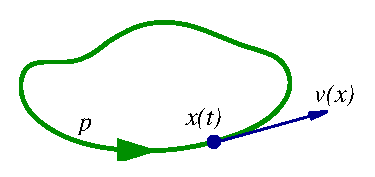
\includegraphics[width=4.0cm]{porbit}
\caption{
 (a) A continuous closed path.
 (b) A smooth loop $\Loop$ with its tangent velocity vector $\lVeloc$.
 (c) A periodic orbit $p$ defined by the vector field $\pVeloc(\ssp)$.
        }
\label{relax:f:loops1}
\end{figure}
%%%%%%%%%%%%%%%%%%%%%%%%%%%%%%%%%%%%%%%%%%%%%%%%%%%%%%%%%%%%%%%%%%
%
% from ChaosBook.org \Chapter{relax}{29mar2004}
\begin{itemize}
  \item[(a)]  {\bf Closed path:}
any closed (not necessarily differentiable) continuous curve $J \subset
\pS$.

  \item[(b)]
{\bf Loop:} a smooth, differentiable closed curve $\lSpace(s)\in \Loop
\subset \pS$, parameterized by $s \in [0,2\pi]$ with
$\lSpace(s)=\lSpace(s+2\pi)$, with the magnitude of the loop tangent
vector fixed by the (so far arbitrary) parametrization of the loop,
\[
\lVeloc(\lSpace)=\frac{d \lSpace}{ds}\,, \quad \lSpace=\lSpace(s) \in \Loop
\,.
\]

  \item[(c)]
{\bf \Po:} given a smooth vector field
 $\pVeloc=\pVeloc(\ssp),\; (\ssp,\pVeloc) \in {\bf T} \pS$,
 periodic orbit $\ssp(t) \in \pS_p$ is a solution of
\[
\frac{dx}{dt}=\pVeloc(\ssp)
    \,,\quad
    \mbox{ such that } \ssp(t)=\ssp(t+\period{p}),
\]
where $\period{p}$ is the shortest period of $p$.

\end{itemize}

\subsection{Gauge transformations}
\label{sec:GaugeTransf}

A change in the choice of `standard located shape' $\tilde{\ssp}$
amounts to a change (rigid motion) of the initial standard shape $\sspRed$,
\beq
\tilde{\ssp} = \Omega(\sspRed) \sspRed
\,.
\ee{ShWiLocalRot}
where $\Omega(\sspRed) \in \Group$ is a \emph{local} transformation, meaning that
every `standard located shape' $\sspRed$ can be transformed by a different
$\Omega$.
As the assignment of `standard located shapes' $\sspRed$ is arbitrary, the
physical results are independent of this assignment,
\refeq{ShWiMovFrame} and \refeq{ShWiLocalRot} imply
that
\beq
\tilde{\LieEl}(\zeit) = {\LieEl}(\zeit)\,\Omega^{-1}\left[\sspRed(\zeit)\right]
\,.
\ee{ShWiNewFrame}
The connecting path integral then transforms as
\beq
\tilde{\LieEl}_{12} = \Omega_{1}\LieEl_{12}\Omega^{-1}_{2}
\,.
\ee{ShWiWilson}
Infinitesimal time step in \refeq{ShWiNewFrame} yields the
the transformation law for $\mathbb{A}$,
\beq
\tilde{\mathbb{A}} = \Omega{\mathbb{A}}\Omega^{-1}
    +\Omega\frac{d\Omega^{-1}}{d\zeit}
\,,
\ee{ShWiGaugeTransf}
where $\Omega_{i}= \Omega[\sspRed(\zeit_i)]$.

In electromagnetism and gauge theories such as Yang-Mills and gravity,
the gauge potential $\mathbb{A}$ describes the translation and rotation resulting
from an arbitrary infinitesimal deformation of a shape (field
configuration).
%
%\item[2013-12-05 Predrag] Faddeev\rf{Faddeev09} writes:
The classical Yang-Mills field $A_\mu(x)=A_\mu^a(x)t^a$
has a geometrical interpretation as a connection in the principal bundle $E=M_4 \times \Group$ where $M_4$ is the Minkowski spacetime, fiber $\Group$ is a compact Lie group, $\mu$ is the Minkowski index
and $t^a$ is a local orthonormal basis in the Lie algebra
\LieAlg\ of \Group\ (the generators $t^a$ of \LieAlg).
In electrodynamics $\Group=\Un{1}$, while in Quantum ChromoDynamics $\Group=\SUn{3}$.

The gauge group $\prod_x \Group$ , consisting of elements $\LieEl(x)$ with values in $\Group$, defines a local change of basis in the fiber,
\beq
t^a = \Omega^{-1}(x) t^a
\,.
\ee{LDFLocalRot}
The action of the gauge group on the connection $A_\mu^a(x)$  is given by
\beq
A_\mu \to A_\mu^\Omega = \Omega A_\mu\Omega^{-1}
    +\Omega\frac{d\Omega^{-1}}{d\mu}
\,.
\ee{LDFgaugeTransf}


For a swimmer
$\mathbb{A}$ takes its values in the Lie
algebra of rigid motions in Euclidean space.
Finite motions are accrued through sequences of infinitesimal shape changes.
To find the translation and rotation of
a swimmer which changes its shape along a given path in shape space, one computes
the path-ordered exponential integral of the gauge potential $\mathbb{A}$ along this path.

In field theory
$\Omega(\sspRed)$ is called a `gauge transformation' in the space of field
configurations; $\mathbb{A}$ transforms as a gauge potential and
the accrued rigid motion
$\LieEl_{12}$ as a Wilson line integral. These are all statements about
classical fields, not about classical or quantum mechanics. The freedom in choosing the `standard located shapes'
$\sspRed$ is the freedom of gauge choice on the space of standard
shapes. The relationship between physical shapes $\ssp(\zeit_2)$
and $\ssp(\zeit_1)$ is manifestly independent of such choices.

\subsection{Shape space as a fibre bundle}
\label{sec:shapeFbundle}
% Shapere \& Wilczek\rf{ShWi06} Appendix A.

In the language of geometry, we are studying \pS\ of shapes in $\reals^d$ and
its quotient modulo the Euclidean group, $\pS/E(3)$.
\pS\ is the bundle, $E(3)$ the fibre, and $\pS/E(3)$ the
base space. Given a path of
(unlocated) shapes in $\pS/E(3)$, the problem is to lift to a path of
shapes with locations in \pS. Dynamical equations determine the local rule
for lifting the path, via the integral over the gauge potential $\mathbb{A}$.
$\mathbb{A}$ tells us the net velocity of the shape through the \statesp\
corresponding to an infinitesimal change of shape. $\mathbb{A}$ is a connection, a linear map from the tangent
space of the base space $T (\pS/E(3))$, to the Lie algebra of $E(3)$.
$\mathbb{A}$ is defined only locally, relative to a local \slice. The
transport of shapes is defined globally. It is the defining property of
\Group-bundles that under a change of \slice, $\sspRed \to
\Omega(\sspRed) \sspRed$, a connection transforms as
\refeq{ShWiGaugeTransf},
\beq
\mathbb{A} \to \Omega{\mathbb{A}}\Omega^{-1}
    +\Omega d\Omega^{-1}
\,.
\ee{ShWiGaugeTransf1}
% clipped from en.wikipedia.org/wiki/Gribov_ambiguity
Gauge fixing means choosing a representative from each gauge orbit. The
space of representatives is a submanifold and represents the gauge fixing
condition. Ideally, every gauge orbit will intersect this submanifold
once and only once. This is generally impossible globally, especially for
non-abelian gauge theories, because of topological obstructions and the
best that can be done is make this condition true locally. A gauge fixing
submanifold may not intersect a gauge orbit at all or it may intersect it
more than once. This is called a Gribov\rf{Gribov77} ambiguity.

\subsection{How to slice}
\label{sec:HowSlice}

%\PC{2013-12-05 Predrag] van Baal\rf{vanBaal97}}

The set of gauge orbits ${\cal A}/\Group$, ${\cal A}$
is the collection of connections, $\Group$ the group of local gauge transformations.

Most frequently, coordinates of this orbit
space are chosen by picking a representative gauge field on the orbit in a smooth and
preferably unique way. Linear gauge conditions like the
Landau or Coulomb gauge suffer from Gribov ambiguities.
In principle therefore, one can introduce different coordinate patches with
transition functions to circumvent this problem.

An (almost) unique representative of the gauge orbit is found by minimizing the
L2 norm of the vector potential along the gauge orbit
    \PC{why $d^3x$?}
\beq
\Norm{A}^2(\LieEl) = \int d^3x \tr\left[\left(\LieEl A_\mu\LieEl^{-1}
    +\LieEl\frac{d}{d\mu}\LieEl^{-1}\right)^2\right]
\,.
\ee{vanBaalnormPotent}
Expanding around the minimum of
\refeq{vanBaalnormPotent}, writing $\LieEl(x) = \exp(\mathbb{A}(x))$, one finds
\bea
\Norm{A}^2(\LieEl) &=& \Norm{A}^2
    + 2 \int d^3x \tr\left(\mathbb{A}\partial_j {A}_j \right)
        \ceq
    + \int d^3x \tr\left(
      \mathbb{A}^\dagger FP(\mathbb{A}) \mathbb{A}\right) + O(\mathbb{A})
\,,
\label{vanBaalnormPotent1}
\eea
where
\beq
FP(\mathbb{A}) = - \partial_j D_j = - \partial_j^2 - \partial_j ad(\mathbb{A}_j)
\,.
\ee{vanBaalFP}
is the Faddeev-Popov operator ($ad(\mathbb{A})X = [\mathbb{A},X]$). At
any local minimum the vector potential is therefore transverse,
$\partial_j {A}_j = 0$, and $FP(\mathbb{A})$ is a positive operator. The
set of all these vector potentials is by definition the Gribov region
$\Omega$. Using the fact that $FP(\mathbb{A})$ is linear in $\mathbb{A}$,
is seen to be a convex subspace of the set of transverse connections. Its
boundary  $\partial\Omega$ is called the Gribov horizon. At the Gribov
horizon, the \emph{lowest} eigenvalue of the Faddeev-Popov operator
vanishes, and points on $\partial\Omega$ are hence associated with
coordinate singularities. Any point on $\partial\Omega$ can be seen to
have a finite distance to the origin of field space.

The Gribov region is the set of local minima of the norm functional
\refeq{vanBaalnormPotent} and needs to be further restricted to the
absolute minima to form a fundamental domain, which will be denoted by
$\Lambda$. The fundamental domain is clearly contained within the Gribov
region.

 	Privatdozent Dr. habil.
 \HREF{http://www.tpi.uni-jena.de/~axm/} {Axel Maas} is cute - has a blog.
He also finds gauge invariance a \HREF{http://axelmaas.blogspot.com/2013/09/blessing-and-bane-redundancy.html}
{blessing and bane}.
In it, \arXiv{1309.1957}, a paper with one of the worst abstracts
ever written, is explained in gentle terms. Some snippets from the article:

``
The minimal Landau gauge\rf{Maas11se} is obtained by minimizing the Hilbert square norm
\beq
|| A ||^2 = \int | A_\mu^b(x) |^2 d^4x,
\eeq
to some local minimum (in general not an absolute minimum) with respect to local gauge transformations $g(x)$.  These act according to ${^g}A_\mu = g^{-1} A_\mu g + g^{-1} \p_\mu g$.  At a local minimum, the functional $F_A(g) \equiv ||{^g}A||^2$ is stationary and its second variation is positive.  It is well known that these two properties imply respectively that the Landau gauge (transversality) condition is satisfied, $\p \cdot A = 0$, and that the Faddeev-Popov operator is positive {\it i. e.} $(\omega, M(A) \omega) \geq 0$ for all $\omega$.  Here the Faddeev-Popov operator acts according to
\beq
\label{Macts}
M^{ac}(A) \omega^c = -  D_\mu^{ac}(A) \p_\mu \omega^c,
\eeq
where the gauge covariant derivative is defined by $D_\mu^{ac}(A) \omega^c = \p_\mu \omega^a + f^{abc} A_\mu^b \omega^c$, and the coupling constant has been absorbed into $A$.  Configurations $A$ that satisfy these two conditions are said to be in the (first) Gribov region\rf{Gribov77} which we designate by $\Omega$.  It is known\rf{Maas11se} that in general there are more than one local minimum of $F_A(g)$, and we do not specify which local minimum is achieved.  This gauge is realized numerically by minimizing a lattice analog of $F_A(g)$ by some algorithm, and the local minimum achieved is in general algorithm dependent. However, for all commonly employed algorithms this does not yield different expectation values, as they all are equivalent to an averaging over the first Gribov region\rf{Maas11se} {Maas:2013vd}.
''




\section{Faddeev-Popov ghosts}
\label{sec:FaddPop}
%\item[2010-09-28 ES: Faddeev-Popov ghosts]


`` %\begin{ttfamily}
It was clear that the equivalence principle had to be taken into account.
In the functional integral framework, the equivalence principle implies
that one has to integrate over classes of gauge equivalent fields instead
of integrating over all fields $A_\mu^a$.

The choice of the representatives in the classes of equivalent fields is
realized by means of a gauge condition (gauge fixing), for instance,
\[
    \partial_{\mu} A_{\mu}^{a} = 0 .
\]
This condition defines a plane in the set of all fields, which is
intersected by the gauge orbits defined by
\[
    A_{\mu} = A_{\mu}^{a}t_{a} \to A_{\mu}^{\Omega}
            = \Omega A_{\mu} \Omega^{-1} + \partial_{\mu} \Omega \Omega^{-1} .
\]
In this context, the difference among abelian and non-abelian cases
becomes clear. In the abelian case, we take $\Omega(x) =
\exp{i\Lambda(x)}$ and a gauge orbit is defined by
\[
    A_{\mu} \to A_{\mu} + \partial_{\mu} \Lambda ,
\]
which is just a linear shift. Thus all the abelian orbits intersect the
gauge surface at the same angle.

In the non-abelian case, the gauge orbit equations are non-linear and the
intersection angle depends on the field parameterizing the orbit. It is
clear that this must be taken into account in the functional integral.
'' %\end{ttfamily}


\Remarks

\remark{Fleeting shapes.}{
\refSect{sec:shapesp} is based on Shapere \& Wilczek
kinematic framework for self-propulsion\rf{ShWi06}, with
equations are rewritten in the notation of
\refref{DasBuch} and
\refref{FrCv11}, Sect.~{\em Dynamics within a slice}.
The results were
announced\rf{ShWi87,ShWi89} in 1987, but the long version\rf{ShWi06}
had to wait for 6 years to be finally accepted in
2006. The authors
were not professional plumbers, but {\em J. Fluid. Mech.}  editors might have
been swayed once Frank Wilczek
got the Nobel Prize, and let that one pass.
%\label{sec:mslices}
    \PC{One might start with `Kinematics = foliation of the \statesp\
        by the symmetry group' vs. `Dynamics = laws of temporal evolution
        (for creationists: `change in time').}
}

\remark{Faddeev-Popov ghosts}{
\refSect{sec:FaddPop} follows Faddeev who in  \refref{Faddeev09}
discusses the difficulties in Yang-Mills quantization that led him
and Popov to introduce fictitious fields, now known as {Faddeev-Popov ghosts}.
They were introduced in the construction of a manifestly Lorentz
covariant quantization of the Yang-Mills field.
The problem was that of gauge fixing, essentially of working on a slice.
We found also 	Privatdozent Dr. habil. \HREF{http://www.tpi.uni-jena.de/~axm/} {Axel Maas} \HREF{http://axelmaas.blogspot.com/2013/09/blessing-and-bane-redundancy.html} {blog} an inspiration, as well as van Baal\rf{vanBaal97}. For a ``Brief history of gauge invariance'', see Zinn-Justin \& Guida\rf{Z-JG08}.
    }

\remark{Method of connections}{
%{\bf [2011-07-08 Predrag]} from \refref{FrCv11}:
%\\
% At this point
It is worth noting that imposing the global and fixed slice
%\refeq{PCsectQ}
is not the only way to separate equivariant dynamics into `rigid
motions' and `shape' dynamics\rf{BeTh04}. In modern mechanics and even
field theory (where elimination of group-directions is called
`gauge-fixing') it is natural to separate the flow {\em locally} into
group dynamics and a transverse, `horizontal'
flow\rf{Smale70I,AbrMars78}, by the `method of
connections'\rf{rowley_reduction_2003}. From our point of view, this
approach is not useful, as they do not reduce the dynamics to a
lower-dimensional \reducedsp\ $\pS/\Group$.
}

\RemarksEnd

\newpage
\begin{description}

\item[2012-02-19 Dan Goldman]
Please read the two Shapere-Wilczek papers\rf{ShWi87,ShWi06} on the
geometric approach to low Re swimming, and the engineering paper from my
CMU colleagues Hatton and Choset\rf{HaCho10} (click
\HREF{http://www.cs.cmu.edu/afs/cs.cmu.edu/Web/People/biorobotics/papers/DSCC2010_Hatton_Choset.pdf}
{here}). We have a paper in submission to PNAS (we are answering some
reviews) which applies these methods to a granular 3 link swimmer,
despite the fact that we don't have an equivalent of NS equations for
granular media. Using our empirical granular drag laws, the CMU guys
predict the optimal forward and turning movements for a 3-link swimmer to
10\% even at high joint angular excursions. I'm presently refining the
paper and making it readable (a reviewer complaint) and I'll send it
along once I do so.

I could really use a physicist to help interpret and help us (me + CMU
guys) take the next step.


\item[2012-02-19, 2013-12-05 Predrag]
I have now read
Koiller, Ehlers, and Montgomery\rf{KoEhlMo96} review. It focuses on the fluid
dynamics aspects of swimming, nothing new compared to Shapere-Wilczek.

Check \refref{ShWi89a,DeArKo04}?

Belot\rf{Belot03} \emph{Symmetry and gauge freedom} is pretty heavy on
formalism, and very heavy on footnotes (history of physics journal). It
is a long slog, and `simple examples' are not that simple - they are
Hamiltonian. But his philosophy rants are fun to read.

``Thus in our examples there is a considerable gain in mathematical tractability in
working with the extended configuration space rather than the reduced configuration
space. It is no surprise that these theories were first written down as constrained
theories with gauge freedom--nor that it continues, for the most part, to be
worthwhile to put up with this gauge freedom rather than struggle with the
conceptually simpler, but technically unpleasant, reduced formulations of the
theories.''

\item[2013-11-14 Predrag]
See also \refchap{c-DailyBlog} {\bf [2010-03-04 Predrag]} on Littlejohn
and M. Reinsch\rf{LiRe97} (click
\HREF{http://ChaosBook.org/library/LiRe97.pdf} {here}).


\item[2012-02-19 Greg Huber]
If you are asking if I can solve their problem, the answer is ``Yes'', I
am sort of an expert on this sort of thing! I have a paper\rf{HuKoYa11}
{\em Micro-swimmers with hydrodynamic interactions} on precisely this
topic. Here is the abstract and a
\HREF{http://www.itp.ucsb.edu/sites/default/files/Huber-Koehler-Yang.pdf}
{link} (or
\HREF{http://ChaosBook.org/library/HuKoYa11.pdf}{click here}):

Abstract:  The low-Reynolds-number motions of Purcell's three-link
swimmer, and of a closely related two-paddle swimmer, are investigated
and compared using slender-body theory and resistive-force theory. The
results are compared (in the case of the three-link swimmer) with the
resistive-force calculations of Becker, Koehler and Stone\rf{BeKoSt03}
(BKS). In particular, we examine the effect of hydrodynamic interaction
and slenderness on the displacement and efficiency of the swimmers. The
BKS analysis is, for the most part, confirmed and extended. However,
deviations of up to 43\% are found in cases where the swimmer propels
itself with large stroke angles. Finally, we discuss recent experimental
data in light of our numerical results.

Also, there is our PRL on Spiroplasma\rf{YaWoHu09} which has some
similarities to a three-link swimmer (click
\HREF{www.itp.ucsb.edu/sites/default/files/Huber-Koehler-Yang.pdf}{here},
or
\HREF{http://ChaosBook.org/library/YaWoHu09.pdf}{here}).

\item[2012-06-15 Evangelos]
Faddeev relies on the group being connected to write group action in
exponential form, as Stefan does. $\On{2}$ in Kuramoto-Sivashinsky is
non-abelian so I am worried that there might be more work required. Are
all non-connected compact Lie groups non-abelian and vice versa?

The weight factor Faddeev and Popov introduced might be helpful in
trace-formulas for non-abelian groups.

Something that still confuses me: Is `Faddeev-Popov operator' really the
gauge orbit tangent vector, or is it the group generator? {\bf
[2012-06-15 Predrag]} I think `group generator' would not have enough
information (why should it be position dependent?), so it should be
something like our group orbit tangent vector, except positivity of
eigenvalues sounds like a projection on a given direction across the
slice.


\item[2013-12-03 Predrag]
Perhaps of interest for going beyond linear stability for cyclic
infinitesimal shape motions of an \eqv: the covariant curl $\mathbb{F}$
of $\mathbb{A}$ presumably describes the curvature of the stable /
unstable manifolds. Shapere \& Wilczek\rf{ShWi06} compute it only for
infinitesimal deformations of a 2D circle and 3D cylinder and sphere.

\item[2013-12-03 Predrag] Shapere \& Wilczek\rf{ShWi06} write:
``If it were only a matter of dividing out by translations, the bundle
would be topologically trivial: there is a globally smooth way of
choosing the centre of a shape; namely to take its centre of mass.
However, choosing orientations does not appear to be so trivial. One
might think of aligning the principal axes with the coordinate axes ~ but
in what order? A natural choice is to order them xyx in order of the
magnitudes of the moments of inertia; but an ambiguity arises when two
moments become equal, and it is not clear that a smooth choice is
possible globally.
[...]
The base space $\pS/E(3)$ seems to have a non-trivial topology, which the
bundle inherits. How `twisted' is the connection $\mathbb{A}$? An answer
might provide us with some qualitative insight into the motion of shapes
which undergo large deformations.
''

\item[2013-12-05 Predrag]
Zinn-Justin \& Guida\rf{Z-JG08} write: ``
In classical electromagnetism, the gauge-fixing problem is simply the problem of choosing a representative in the class of equivalent potentials, convenient for practical calculations or most suited to physical intuition.

[...] Indeed, since the integrand in field integrals giving physical observables is constant along gauge orbits (the set of all gauge fields obtained from one representative by gauge transformations), the naive field integrals (sums over all field configurations) are not defined. It becomes necessary to fix the gauge, that is, to integrate only over a section of gauge field space that -ideally- contains only one representative per orbit.

Moreover, it is necessary to integrate over gauge fields with a measure ensuring that physical results are independent of the choice of the section. Such a measure has been identified by Faddeev and Popov (1967) and, in the case of Landau's gauge, contains as a factor the absolute value of the determinant of a differential operator.

[...] However, the problem of integration over suitable gauge sections is more subtle at a non-perturbative level. Indeed, one would like the section to cut once or, at least, the same number of times all gauge orbits, but this is not generally the case in non-Abelian gauge theories, as first pointed out by Gribov\rf{Gribov77} in (Gribov 1978). (One speaks then of Gribov copies.) In particular, the Faddeev-Popov determinant changes sign when two Gribov copies merge and, if the absolute value of the determinant is not taken into proper account, the integration measure is no longer positive. One idea is then to restrict the integration to the region enclosing only one Gribov copy, but this is not easy to achieve in practice.
''



\end{description}


\renewcommand{\sspRed}{\ensuremath{\hat{\ssp}}}
\renewcommand{\LieEl}{\ensuremath{\gamma}}  % also a Siminos Lie group element
